\chapter{Getting Started}
\label{ch:gettingstarted}

This Getting Started guide is written with a default installation in mind, meaning that some parts may not apply if a custom installation was used.
When the \textit{allpix} binary is used, this refers to the executable installed in \text{bin/allpix} in the installation path.
It is worth noting that before running any \apsq simulation, ROOT and (in most cases) Geant4 should be initialized.
Refer to Section~\ref{sec:initialize_dependencies} for instructions on how to load these libraries.

\section{Configuration Files}
\label{sec:configuration_files}
The framework is configured with simple human-readable configuration files.
The configuration format is described in detail in Section~\ref{sec:config_file_format}, and consists of several section headers within $[$ and $]$ brackets, and a section without header at the start.
Each of these sections contains a set of key/value pairs separated by the \texttt{=} character.
Comments are indicated using the hash symbol (\texttt{\#}).

The framework has the following three required layers of configuration files:
\begin{itemize}
\item The \textbf{main} configuration: The most important configuration file and the file that is passed directly to the binary.
Contains both the global framework configuration and the list of modules to instantiate together with their configuration.
An example can be found in the repository at \textit{examples/example.conf}.
More details and a more thorough example are found in Section~\ref{sec:main_config}, several advanced simulation chain configurations are presented in Chapter~\ref{ch:examples}.
\item The \textbf{geometry} configuration passed to the framework to determine the detector setup and passive materials.
Describes the detector setup, containing the position, orientation and model type of all detectors.
Optionally, passive materials can be added to this configuration.
Examples are available in the repository at \file{examples/example_detector.conf} or \file{examples/example_detector_passive.conf}.
Introduced in Section~\ref{sec:detector_config}.
\item The detector \textbf{model} configuration.
Contains the parameters describing a particular type of detector.
Several models are already provided by the framework, but new types of detectors can easily be added.
See \textit{models/test.conf} in the repository for an example.
Please refer to Section~\ref{sec:adding_detector_model} for more details about adding new models.
\end{itemize}

In the following paragraphs, the available types and the unit system are explained and an introduction to the different configuration files is given.

\subsection{Parsing types and units}
\label{sec:config_values}
The \apsq framework supports the use of a variety of types for all configuration values.
The module specifies how the value type should be interpreted.
An error will be raised if either the key is not specified in the configuration file, the conversion to the desired type is not possible, or if the given value is outside the domain of possible options.
Please refer to the module documentation in Chapter~\ref{ch:modules} for the list of module parameters and their types.
Parsing the value roughly follows common-sense (more details can be found in Section~\ref{sec:accessing_parameters}).
A few special rules do apply:
\begin{itemize}
\item If the value is a \textbf{string}, it may be enclosed by a single pair of double quotation marks (\texttt{"}), which are stripped before passing the value to the modules.
If the string is not enclosed by quotation marks, all whitespace before and after the value is erased.
If the value is an array of strings, the value is split at every whitespace or comma (\texttt{,}) that is not enclosed in quotation marks.
\item If the value is a \textbf{boolean}, either numerical (\texttt{0}, \texttt{1}) or textual (\texttt{false}, \texttt{true}) representations are accepted.
\item If the value is a \textbf{relative path}, that path will be made absolute by adding the absolute path of the directory that contains the configuration file where the key is defined.
\item If the value is an \textbf{arithmetic} type, it may have a suffix indicating the unit.
The list of base units is shown in Table~\ref{tab:units}.
\end{itemize}

\begin{warning}
  If no units are specified, values will always be interpreted in the base units of the framework.
  In some cases this can lead to unexpected results.
  E.g. specifying a bias voltage as \texttt{bias\_voltage = 50} results in an applied voltage of \SI{50}{\mega\volt}.
  Therefore it is strongly recommended to always specify units in the configuration files.
\end{warning}

The internal base units of the framework are not chosen for user convenience but for maximum precision of the calculations and in order to avoid the necessity of conversions in the code.

\begin{table}[tbp]
\caption{List of units supported by \apsq}
\label{tab:units}
\centering
\begin{tabular}{lll}
  \toprule
\textbf{Quantity}                 & \textbf{Default unit}                   & \textbf{Auxiliary units} \\
 \midrule
 \textit{Unity}                   & 1                                       & ---                      \\
 \midrule
 \multirow{6}{*}{\textit{Length}} & \multirow{6}{*}{mm (millimeter)}        & nm (nanometer)           \\
                                  &                                         & um (micrometer)          \\
                                  &                                         & cm (centimeter)          \\
                                  &                                         & dm (decimeter)           \\
                                  &                                         & m (meter)                \\
                                  &                                         & km (kilometer)           \\
 \midrule
\multirow{4}{*}{\textit{Time}}    & \multirow{4}{*}{ns (nanosecond)}        & ps (picosecond)          \\
                                  &                                         & us (microsecond)         \\
                                  &                                         & ms (millisecond)         \\
                                  &                                         & s (second)               \\
\midrule
\multirow{3}{*}{\textit{Energy}}  & \multirow{3}{*}{MeV (megaelectronvolt)} & eV (electronvolt)        \\
                                  &                                         & keV (kiloelectronvolt)   \\
                                  &                                         & GeV (gigaelectronvolt)   \\
\midrule
\textit{Temperature}              & K (kelvin)                              & ---                      \\
\midrule
\multirow{3}{*}{\textit{Charge}}  & \multirow{3}{*}{e (elementary charge)}  & ke (kiloelectrons)       \\
                                  &                                         & fC (femtocoulomb)        \\
                                  &                                         & C (coulomb)              \\
\midrule
\multirow{2}{*}{\textit{Voltage}} & \multirow{2}{*}{MV (megavolt)}          & V (volt)                 \\
                                  &                                         & kV (kilovolt)            \\
\midrule
\textit{Magnetic field strength}  & T (tesla)                               & mT (millitesla)          \\
\midrule
\multirow{2}{*}{\textit{Angle}}   & \multirow{2}{*}{rad (radian)}           & deg (degree)             \\
                                  &                                         & mrad (milliradian)       \\
\bottomrule
\end{tabular}
\end{table}

Combinations of base units can be specified by using the multiplication sign \texttt{*} and the division sign \texttt{/} that are parsed in linear order (thus $\frac{V m}{s^2}$ should be specified as $V*m/s/s$).
The framework assumes the default units (as given in Table~\ref{tab:units}) if the unit is not explicitly specified.
It is recommended to always specify the unit explicitly for all parameters that are not dimensionless as well as for angles.

Examples of specifying key/values pairs of various types are given below:
\begin{minted}[frame=single,framesep=3pt,breaklines=true,tabsize=2,linenos]{ini}
# All whitespace at the front and back is removed
first_string =   string_without_quotation
# All whitespace within the quotation marks is preserved
second_string = "  string with quotation marks  "
# Keys are split on whitespace and commas
string_array = "first element" "second element","third element"
# Elements of matrices with more than one dimension are separated
# using square brackets
string_matrix_3x3 = [["1","0","0"], ["0","cos","-sin"], ["0","sin",cos]]
# If the matrix is of dimension 1xN, the outer brackets have to be
# added explicitly
integer_matrix_1x3 = [[10, 11, 12]]
# Integer and floats can be specified in standard formats
int_value = 42
float_value = 123.456e9
# Units can be passed to arithmetic types
energy_value = 1.23MeV
time_value = 42ns
# Units are combined in linear order without grouping or implicit brackets
acceleration_value = 1.0m/s/s
# Thus the quantity below is the same as 1.0deg*kV*K/m/s
random_quantity = 1.0deg*kV/m/s*K
# Relative paths are expanded to absolute paths, e.g. the following value
# will become "/home/user/test" if the configuration file is located
# at "/home/user"
output_path = "test"
# Booleans can be represented in numerical or textual style
my_switch = true
my_other_switch = 0
\end{minted}

\subsection{Main configuration}
\label{sec:main_config}
The main configuration consists of a set of sections specifying the modules used.
All modules are executed in the \emph{linear} order in which they are defined.
There are a few section names which have a special meaning in the main configuration, namely the following:
\begin{itemize}
\item The \textbf{global} (framework) header sections: These are all zero-length section headers (including the one at the beginning of the file) and all sections marked with the header \parameter{[Allpix]} (case-insensitive).
These are combined and accessed together as the global configuration, which contain all parameters of the framework itself (see Section~\ref{sec:framework_parameters} for details).
All key-value pairs defined in this section are also inherited by all individual configurations as long the key is not defined in the module configuration itself.
\item The \textbf{ignore} header sections: All sections with name \parameter{[Ignore]} (case-insensitive) are ignored.
Key-value pairs defined in the section as well as the section itself are discarded by the parser.
These section headers are useful for quickly enabling and disabling individual modules by replacing their actual name by an ignore section header.
\end{itemize}

All other section headers are used to instantiate modules of the respective name.
Installed modules are loaded automatically.
If problems arise please review the loading rules described in Section~\ref{sec:module_instantiation}.

Modules can be specified multiple times in the configuration files, depending on their type and configuration.
The type of the module determines how the module is instantiated:
\begin{itemize}
\item If the module is \textbf{unique}, it is instantiated only a single time irrespective of the number of detectors.
These kinds of modules should only appear once in the whole configuration file unless different inputs and outputs are used, as explained in Section~\ref{sec:redirect_module_input_outputs}.
\item If the module is \textbf{detector}-specific, it is instantiated once for every detector it is configured to run on.
By default, an instantiation is created for all detectors defined in the detector configuration file (see Section~\ref{sec:detector_config}, lowest priority) unless one or both of the following parameters are specified:
\begin{itemize}
\item \parameter{name}: An array of detector names the module should be executed for.
Replaces all global and type-specific modules of the same kind (highest priority).
\item \parameter{type}: An array of detector types the module should be executed for.
Instantiated after considering all detectors specified by the name parameter above.
Replaces all global modules of the same kind (medium priority).
\end{itemize}
Within the same module, the order of the individual instances in the configuration file is irrelevant.
\end{itemize}

A valid example configuration using the detector configuration above is:
\begin{minted}[frame=single,framesep=3pt,breaklines=true,tabsize=2,linenos]{ini}
# Key is part of the empty section and therefore the global configuration
string_value = "example1"
# The location of the detector configuration is a global parameter
detectors_file = "manual_detector.conf"
# The Allpix section is also considered global and merged with the above
[Allpix]
another_random_string = "example2"

# First run a unique module
[MyUniqueModule]
# This module takes no parameters
# [MyUniqueModule] cannot be instantiated another time

# Then run detector modules on different detectors
# First run a module on the detector of type Timepix
[MyDetectorModule]
type = "timepix"
int_value = 1
# Replace the module above for `dut` with a specialized version
# It does not inherit any parameters from earlier modules
[MyDetectorModule]
name = "dut"
int_value = 2
# Run the module on the remaining unspecified detector (`telescope1`)
[MyDetectorModule]
# int_value is not specified, so it uses the default value
\end{minted}

In the following paragraphs, a fully functional (albeit simple) configuration file with valid configuration is presented, as opposed to the above examples with hypothetical module names for illustrative purpose.

\subsection{Detector configuration}
\label{sec:detector_config}
The detector configuration consists of a set of sections describing the detectors in the setup.
Each section starts with a header describing the name used to identify the detector; all names are required to be unique.
Every detector has to contain all of the following parameters:
\begin{itemize}
\item A string referring to the \parameter{type} of the detector model.
The model should exist in the search path described in Section~\ref{sec:detector_models}.
\item The 3D \parameter{position} in the world frame in the order x, y, z.
See Section~\ref{sec:models_geometry} for details.
\item The \parameter{orientation} specified as X-Y-Z extrinsic Euler angles.
This means the detector is rotated first around the world's X-axis, then around the world's Y-axis and then around the world's Z-axis.
Alternatively the orientation can be set as Z-Y-X or X-Z-X extrinsic Euler angles, refer to Section~\ref{sec:models_geometry} for details.
\end{itemize}

In addition to these required parameters, the following parameters allow to randomly misalign the respective detector from its initial position. The values are interpreted as width of a normal distribution centered around zero.
In order to reproduce misalignments, a fixed random seed for the framework core can be used as explained in Section~\ref{sec:framework_parameters}.
Misalignment can be introduced both for shifts along the three global axes and the three rotations angles with the following parameters:
\begin{itemize}
\item The parameter \parameter{alignment_precision_position} allows the specification of the alignment precision along the three global axes. Each value represents the Gaussian width with which the detector will be randomly misaligned along the corresponding axis.
\item The parameter \parameter{alignment_precision_orientation} allows to specify the alignment precision in the three rotation angles defined by the \parameter{orientation} parameter. The misalignments are added to the individual angles before combining them into the final rotation as defined by the \parameter{orientation_mode} parameter.
\end{itemize}

The optional parameter \parameter{role} accepts the values \parameter{active} for detectors and \parameter{passive} for passive elements in the setup.
If no value is given, \parameter{active} is taken as the default value.

Furthermore it is possible to specify certain parameters of the detector explained in more detail in Section~\ref{sec:detector_models}.
This allows to quickly adapt e.g. the sensor thickness of a certain detector without altering the actual detector model file.

\begin{figure}[t]
  \centering
  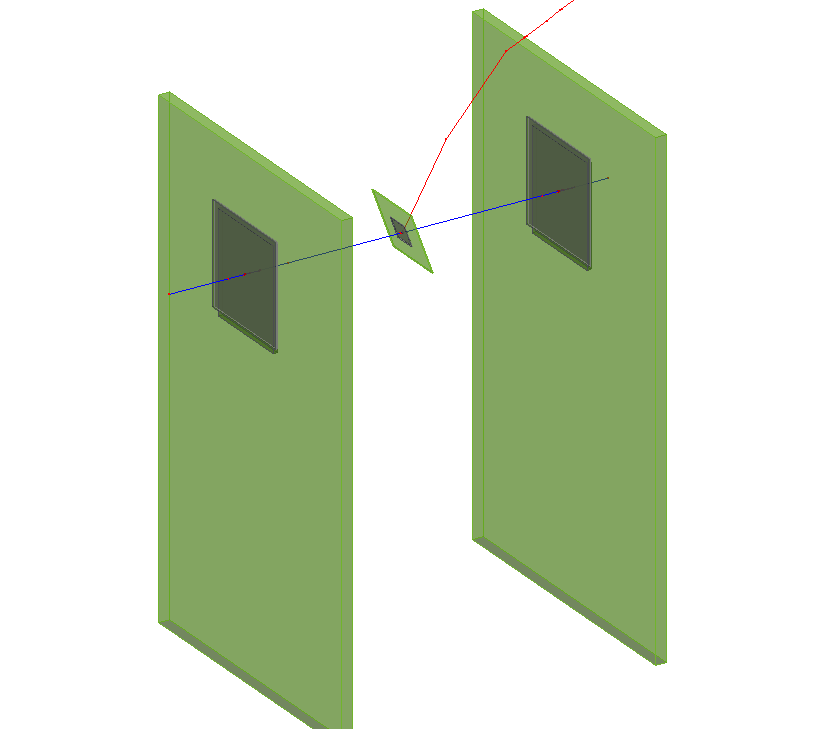
\includegraphics[width=0.6\textwidth]{telescope.png}
  \caption{Visualization of a Pion passing through the telescope setup defined in the detector configuration file. A secondary particle is produced in the material of the detector in the center.}
  \label{fig:telescope}
\end{figure}

An example configuration file describing a setup with one CLICpix2 detector and two Timepix~\cite{timepix} models is the following:
\inputminted[frame=single,framesep=3pt,breaklines=true,tabsize=2,linenos]{ini}{../../etc/manual_detector.conf}
Figure~\ref{fig:telescope} shows a visualization of the setup described in the file.
This configuration is used in the rest of this chapter for explaining concepts.

\subsubsection{Passive material configuration}
\label{sec:passive_material_config}

Descriptions of passive materials can be added to the detector setup via a set of sections, with a syntax similar to the detector configuration.
Passive geometry entries are identified by the \parameter{role} parameter set to \parameter{passive}.
Each section starts with a header describing the name used to identify the passive material; all names are required to be unique.

Every passive material has to contain all of the following parameters:
\begin{itemize}
  \item The \parameter{position} and \parameter{orientation} of the material as described for the detector, see Section \ref{sec:detector_config}.
  \item A string referring to the \parameter{type} of the passive material.
  The model should be interpreted by the module constructing the passive material, such as for example the GeometryBuilderGeant4 module.
  \item A string referring to the \parameter{material} of the passive material.
  The materials are defined in the GeometryBuilderGeant4 module and are described in the module section.
  \item A set of size parameters specific for the model that is chosen.
  All size parameters that describe the total length of something are placed such that half of this total length extends from each side of the given \parameter{position}.
  If a parameter describes the radius, this means the radius will extend from the \parameter{position} on both sides, making its total size two times the radius in the given direction.
  The size parameters for the specific models are described in Section~\ref{geometrybuildergeant4}.
\end{itemize}

In addition, an optional string referring to the \parameter{mother_volume}, which defines another passive material the volume will be placed in, can be specified.
Note: If a mother volume is chosen, the position defined in the configuration file will be relative to the center of the mother volume. An error will be given if the specified mother volume is too small for the specified size or position of this volume. Per default, the mother volume is the world frame.
Note: if the \parameter{mother_volume} is a hollow material, only the non-hollow part of the material is considered part of the material. Placing a passive volume in the hollow part requires a different \parameter{mother_volume}.

Similar to the detector configuration, the parameters \parameter{orientation_mode} (see Section~\ref{sec:models_geometry}), \parameter{alignment_precision_position} and \parameter{alignment_precision_orientation} (see Section~\ref{sec:detector_config}) can be used optionally to define the rotation order and a possible misalignment of passive materials.

An example configuration file describing a set of passive materials with different configuration options is the following:
\inputminted[frame=single,framesep=3pt,breaklines=true,tabsize=2,linenos]{ini}{../../etc/manual_passive_materials.conf}
Figure~\ref{fig:passivematerials} shows a visualization of the setup described in the file.

\begin{figure}[t]
  \centering
  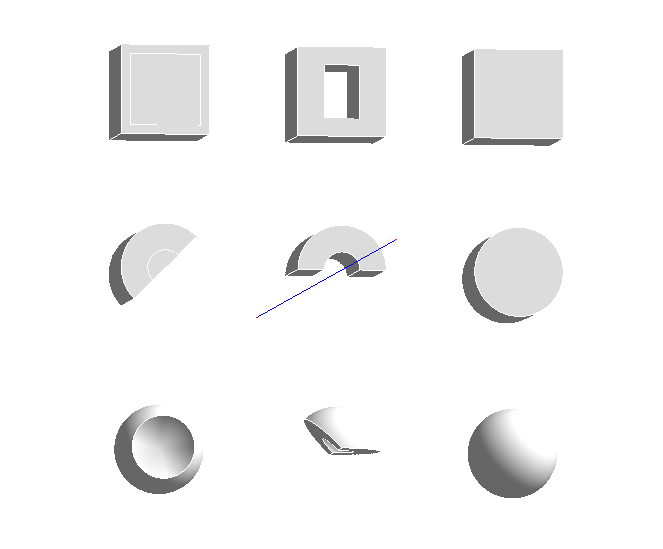
\includegraphics[width=0.6\textwidth]{passive_materials.png}
  \caption{Visualization of a set of passive materials showing different configuration options.}
  \label{fig:passivematerials}
\end{figure}


\section{Framework parameters}
\label{sec:framework_parameters}
The \apsq framework provides a set of global parameters which control and alter its behavior:
\begin{itemize}
\item \parameter{detectors_file}: Location of the file describing the detector configuration (introduced in Section~\ref{sec:detector_config}).
The only \textit{required} global parameter: the framework will fail to start if it is not specified.
\item \parameter{number_of_events}: Determines the total number of events the framework should simulate.
Defaults to one (simulating a single event).
\item \parameter{root_file}: Location relative to the \parameter{output_directory} where the ROOT output data of all modules will be written to. The file extension \texttt{.root} will be appended if not present.
Default value is \textit{modules.root}.
Directories within the ROOT file will be created automatically for all module instantiations.
\item \parameter{log_level}: Specifies the lowest log level which should be reported.
Possible values are \texttt{FATAL}, \texttt{STATUS}, \texttt{ERROR}, \texttt{WARNING}, \texttt{INFO} and \texttt{DEBUG}, where all options are case-insensitive.
Defaults to the \texttt{INFO} level.
More details and information about the log levels, including how to change them for a particular module, can be found in Section~\ref{sec:logging_verbosity}.
Can be overwritten by the \texttt{-v} parameter on the command line (see Section~\ref{sec:allpix_executable}).
\item \parameter{log_format}: Determines the log message format to display.
Possible options are \texttt{SHORT}, \texttt{DEFAULT} and \texttt{LONG}, where all options are case-insensitive.
More information can be found in Section~\ref{sec:logging_verbosity}.
\item \parameter{log_file}: File where the log output should be written to in addition to printing to the standard output (usually the terminal).
Only writes to standard output if this option is not provided.
Another (additional) location to write to can be specified on the command line using the \texttt{-l} parameter (see Section~\ref{sec:allpix_executable}).
\item \parameter{output_directory}: Directory to write all output files into.
Subdirectories are created automatically for all module instantiations.
This directory will also contain the \parameter{root_file} specified via the parameter described above.
Defaults to the current working directory with the subdirectory \textit{output/} attached.
\item \parameter{purge_output_directory}: Decides whether the content of an already existing output directory is deleted before a new run starts. Defaults to \texttt{false}, i.e. files are kept but will be overwritten by new files created by the framework.
\item \parameter{deny_overwrite}: Forces the framework to abort the run and throw an exception when attempting to overwrite an existing file. Defaults to \texttt{false}, i.e. files are overwritten when requested. This setting is inherited by all modules, but can be overwritten in the configuration section of each of the modules.
\item \parameter{random_seed}: Seed for the global random seed generator used to initialize seeds for module instantiations.
The 64-bit Mersenne Twister \command{mt19937_64} from the \CPP Standard Library is used to generate seeds.
A random seed from multiple entropy sources will be generated if the parameter is not specified.
Can be used to reproduce an earlier simulation run.
\item \parameter{random_seed_core}: Optional seed used for pseudo-random number generators in the core components of the framework. If not set explicitly, the value $(\textrm{\parameter{random_seed}} + 1)$ is used.
\item \parameter{library_directories}: Additional directories to search for module libraries, before searching the default paths.
See Section~\ref{sec:module_instantiation} for details.
\item \parameter{model_paths}: Additional files or directories from which detector models should be read besides the standard search locations.
Refer to Section~\ref{sec:detector_models} for more information.
\item \parameter{experimental_multithreading}: Enable \textbf{experimental} multi-threading for the framework. This can speed up simulations of multiple detectors significantly. More information about multi-threading can be found in Section~\ref{sec:multithreading}.
\item \parameter{workers}: Specify the number of workers to use in total, should be strictly larger than zero. Only used if \parameter{experimental_multithreading} is set to true. Defaults to the number of native threads available on the system if this can be determined, otherwise one thread is used.
\end{itemize}

\section{The \textit{allpix} Executable}
\label{sec:allpix_executable}
The \parameter{allpix} executable functions as the interface between the user and the framework. It is primarily used to provide the main configuration file, but also allows to add and overwrite options from the main configuration file. This is both useful for quick testing as well as for batch processing of simulations.

The executable handles the following arguments:
\begin{itemize}
\item \texttt{-c <file>}: Specifies the configuration file to be used for the simulation, relative to the current directory.
This is the only \underline{required} argument, the simulation will fail to start if this argument is not given.
\item \texttt{-l <file>}: Specify an additional location to forward log output to, besides standard output and the location specified in the framework parameters explained in Section~\ref{sec:framework_parameters}.
\item \texttt{-v <level>}: Sets the global log verbosity level, overwriting the value specified in the configuration file described in Section~\ref{sec:framework_parameters}.
Possible values are \texttt{FATAL}, \texttt{STATUS}, \texttt{ERROR}, \texttt{WARNING}, \texttt{INFO} and \texttt{DEBUG}, where all options are case-insensitive.
The module specific logging level introduced in Section~\ref{sec:logging_verbosity} is not overwritten.
\item \texttt{-{}-version}: Prints the version and build time of the executable and terminates the program.
\item \texttt{-o <option>}: Passes extra framework or module options which are added and overwritten in the main configuration file.
This argument may be specified multiple times, to add multiple options.
Options are specified as key/value pairs in the same syntax as used in the configuration files (refer to Section~\ref{sec:config_file_format} for more details), but the key is extended to include a reference to a configuration section or instantiation in shorthand notation.
There are three types of keys that can be specified:
\begin{itemize}
\item Keys to set \textbf{framework parameters}. These have to be provided in exactly the same way as they would be in the main configuration file (a section does not need to be specified). An example to overwrite the standard output directory would be \texttt{allpix -c <file> -o output\_directory="run123456"}.
\item Keys for \textbf{module configurations}. These are specified by adding a dot (\texttt{.}) between the module and the actual key as it would be given in the configuration file (thus \textit{module}.\textit{key}). An example to overwrite the deposited particle to a positron would be \texttt{allpix -c <file> -o DepositionGeant4.particle\_type="e+"}.
\item Keys to specify values for a particular \textbf{module instantiation}. The identifier of the instantiation and the name of the actual key are split by a dot (\texttt{.}), in the same way as for keys for module configurations (thus \textit{identifier}.\textit{key}). The unique identifier for a module can contains one or more colons (\texttt{:}) to distinguish between various instantiations of the same module. The exact name of an identifier depends on the name of the detector and the optional input and output name. Those identifiers can be extracted from the logging section headers. An example to change the temperature of propagation for a particular instantiation for a detector named \textit{dut} could be \texttt{allpix -c <file> -o GenericPropagation:dut.temperature=273K}.
\end{itemize}
Note that only the single argument directly following the \texttt{-o} is interpreted as the option. If there is whitespace in the key/value pair this should be properly enclosed in quotation marks to ensure the argument is parsed correctly.
\item \texttt{-g <option>}: Passes extra detector options which are added and overwritten in the detector configuration file.
This argument can be specified multiple times, to add multiple options.
The options are parsed in the same way as described above for module options, but only one type of key can be specified to overwrite an option for a single detector.
These are specified by adding a dot (\texttt{.}) between the detector and the actual key as it would be given in the detector configuration file (thus \textit{detector}.\textit{key}). This method also works for customizing detector models as described in Section \ref{sec:detector_models}. An example to overwrite the sensor thickness for a particular detector named \texttt{detector1} to \texttt{50um} would be \texttt{allpix -c <file> -g detector1.sensor\_thickness=50um}.
\end{itemize}

No interaction with the framework is possible during the simulation. Signals can however be send using keyboard shortcuts to terminate the simulation, either gracefully or with force. The executable understand the following signals:
\begin{itemize}
    \item SIGINT (\texttt{CTRL+C}): Request a graceful shutdown of the simulation. This means the current simulated event is finished, while all other events requested in the configuration file are ignored. After finishing the event, the finalization stage is run for every module to ensure all modules finish properly. This signal can be very useful when too many events are specified and the simulation takes too long to finish entirely, but the output generated so far should still be kept.
    \item SIGTERM: Same as SIGINT, request a graceful shutdown of the simulation. This signal is emitted e.g.\ by the \command{kill} command or by cluster computing schedulers to ask for a termination of the job.
    \item SIGQUIT (\texttt{CTRL+\textbackslash}): Forcefully terminates the simulation. It is not recommended to use this signal as it will normally lead to the loss of all generated data. This signal should only be used when graceful termination is for any reason not possible.
\end{itemize}


\section{Setting up the Simulation Chain}
\label{sec:setting_up_simulation_chain}

In the following, the framework parameters are used to set up a fully functional simulation.
Module parameters are shortly introduced when they are first used.
For more details about these parameters, the respective module documentation in Chapter~\ref{ch:modules} should be consulted.
A typical simulation in \apsq will contain the following components:
\begin{itemize}

\item The \textbf{geometry builder}, responsible for creating the external Geant4 geometry from the internal geometry.
In this document, \emph{internal geometry} refers to the detector parameters used by \apsq for coordinate transformations and conversions throughout the simulation, while \emph{external geometry} refers to the constructed Geant4 geometry used for charge carrier deposition (and possibly visualization).
\item The \textbf{deposition} module that simulates the particle beam creating charge carriers in the detectors using the provided physics list (containing a description of the simulated interactions) and the geometry created above.
\item A \textbf{propagation} module that propagates the charges through the sensor.
\item A \textbf{transfer} module that transfers the charges from the sensor electrodes and assigns them to a pixel of the readout electronics.
\item A \textbf{digitizer} module which converts the charges in the pixel to a detector hit, simulating the front-end electronics response.
\item An \textbf{output} module, saving the data of the simulation.
The \apsq standard file format is a ROOT TTree, which is described in detail in Section~\ref{sec:storing_output_data}.
\end{itemize}

In this example, charge carriers will be deposited in the three sensors defined in the detector configuration file in Section~\ref{sec:detector_config}.
All charge carriers deposited in the different sensors will be propagated and digitized.
Finally, monitoring histograms for the device under test (DUT) will be recorded in the framework's main ROOT file and all simulated objects, including the entry and exit positions of the simulated particles (Monte Carlo truth), will be stored in a ROOT file using the \apsq format.
An example configuration file implementing this would look like:
\inputminted[frame=single,framesep=3pt,breaklines=true,tabsize=2,linenos]{ini}{../../etc/manual.conf}

This configuration is available in the repository at \file{etc/manual.conf}.
The detector configuration file from Section~\ref{sec:detector_config} can be found at \file{etc/manual_detector.conf}.

The simulation is started by passing the path of the main configuration file to the \parameter{allpix} executable as follows:
\begin{verbatim}
$ allpix -c etc/manual.conf
\end{verbatim}
The detector histograms such as the hit map are stored in the ROOT file \file{output/modules.root} in the TDirectory \textit{DetectorHistogrammer/}.

If problems occur when exercising this example, it should be made sure that an up-to-date and properly installed version of \apsq is used (see the installation instructions in Chapter~\ref{ch:installation}).
If modules or models fail to load, more information about potential issues with the library loading can be found in the detailed framework description in Chapter~\ref{ch:framework}.

\section{Extending the Simulation Chain}
In the following, a few basic modules will be discussed which may be of use during a first simulation.

\paragraph{Visualization}
Displaying the geometry and the particle tracks helps both in checking and interpreting the results of a simulation.
Visualization is fully supported through Geant4, supporting all the options provided by Geant4~\cite{geant4vis}.
Using the Qt viewer with OpenGL driver is the recommended option as long as the installed version of Geant4 is built with Qt support enabled.

To add the visualization, the \parameter{VisualizationGeant4} section should be added at the end of the configuration file.
An example configuration with some useful parameters is given below:
\begin{minted}[frame=single,framesep=3pt,breaklines=true,tabsize=2,linenos]{ini}
[VisualizationGeant4]
# Use the Qt gui
mode = "gui"

# Set transparency of the detector models (in percent)
transparency = 0.4
# Set viewing style (alternative is 'wireframe')
view_style = "surface"

# Color trajectories by charge of the particle
trajectories_color_mode = "charge"
trajectories_color_positive = "blue"
trajectories_color_neutral = "green"
trajectories_color_negative = "red"
\end{minted}
If Qt is not available, a VRML viewer can be used as an alternative, however it is recommended to reinstall Geant4 with the Qt viewer included as it offers the best visualization capabilities.
The following steps are necessary in order to use a VRML viewer:
\begin{itemize}
\item A VRML viewer should be installed on the operating system.
Good options are FreeWRL or OpenVRML.
\item Subsequently, two environmental parameters have to be exported to the shell environment to inform Geant4 about the configuration:
\parameter{G4VRMLFILE_VIEWER} should point to the location of the viewer executable and \parameter{G4VRMLFILE_MAX_FILE_NUM} should typically be set to 1 to prevent too many files from being created.
\item Finally, the configuration section of the visualization module should be altered as follows:
\end{itemize}

\begin{minted}[frame=single,framesep=3pt,breaklines=true,tabsize=2,linenos]{ini}
[VisualizationGeant4]
# Do not start the Qt gui
mode = "none"
# Use the VRML driver
driver = "VRML2FILE"
\end{minted}

More information about all possible configuration parameters can be found in the module documentation in Chapter~\ref{ch:modules}.

\paragraph{Electric Fields}
\label{sec:module_electric_field}
By default, detectors do not have an electric field associated with them, and no bias voltage is applied.
A field can be added to each detector using the \parameter{ElectricFieldReader} module.

The section below calculates a linear electric field for every point in active sensor volume based on the depletion voltage of the sensor and the applied bias voltage.
The sensor is always depleted from the implant side; the direction of the electric field depends on the sign of the bias voltage as described in the module description in Chapter~\ref{ch:modules}.
\begin{minted}[frame=single,framesep=3pt,breaklines=true,tabsize=2,linenos]{ini}
# Add an electric field
[ElectricFieldReader]
# Set the field type to `linear`
model = "linear"
# Applied bias voltage to calculate the electric field from
bias_voltage = -50V
# Depletion voltage at which the given sensor is fully depleted
depletion_voltage = -10V
\end{minted}

\apsq also provides the possibility to utilize a full electrostatic TCAD simulation for the description of the electric field.
In order to speed up the lookup of the electric field values at different positions in the sensor, the adaptive TCAD mesh has to be interpolated and transformed into a regular grid with configurable feature size before use.
\apsq comes with a converter tool which reads TCAD DF-ISE files from the sensor simulation, interpolates the field, and writes this out in an appropriate format.
A more detailed description of the tool can be found in Section~\ref{sec:tcad_electric_field_converter}.
An example electric field (with the file name used in the example below) can be found in the \textit{etc} directory of the \apsq repository.

Electric fields can be attached to a specific detector using the standard syntax for detector binding.
A possible configuration would be:
\begin{minted}[frame=single,framesep=3pt,breaklines=true,tabsize=2,linenos]{ini}
[ElectricFieldReader]
# Bind the electric field to the detector named `dut`
name = "dut"
# Specify that the model is provided as meshed electric field map format, e.g. converted from TCAD
model = "mesh"
# Name of the file containing the electric field
file_name = "example_electric_field.init"
\end{minted}

\paragraph{Magnetic Fields}
\label{sec:module_magnetic_field}

For simulating the detector response in the presence of a magnetic field with \apsq, a constant, global magnetic field can be defined. By default, it is turned off. A field can be added to the whole setup using the unique module \parameter{MagneticFieldReader}, passing the field vector as parameter:
\begin{minted}[frame=single,framesep=3pt,breaklines=true,tabsize=2,linenos]{ini}
# Add a magnetic field
[MagneticFieldReader]
# Constant magnetic field (currently this is the default value)
model="constant"
# Magnetic field vector
magnetic_field = 0mT 3.8T 0T
\end{minted}

The global magnetic field is used by the interface to Geant4 and therefore exposes charged primary particles to the Lorentz force, and as a property of each detector present, enabling a Lorentz drift of the charge carriers in the active sensors, if supported by the used propagation modules. See Chapter \ref{ch:modules} for more information on the available propagation modules.

Currently, only constant magnetic fields can be applied.

\section{Logging and Verbosity Levels}
\label{sec:logging_verbosity}
\apsq is designed to identify mistakes and implementation errors as early as possible and to provide the user with clear indications about the problem.
The amount of feedback can be controlled using different log levels which are inclusive, i.e.\ lower levels also include messages from all higher levels.
The global log level can be set using the global parameter \parameter{log_level}.
The log level can be overridden for a specific module by adding the \parameter{log_level} parameter to the respective configuration section.
The following log levels are supported:
\begin{itemize}
\item \textbf{FATAL}: Indicates a fatal error that will lead to direct termination of the application.
Typically only emitted in the main executable after catching exceptions as they are the preferred way of fatal error handling (as discussed in Section~\ref{sec:error_reporting_exceptions}).
An example of a fatal error is an invalid configuration parameter.
\item \textbf{STATUS}: Important information about the status of the simulation.
Is only used for messages which have to be logged in every run such as the global seed for pseudo-random number generators and the current progress of the run.
\item \textbf{ERROR}: Severe error that should not occur during a normal well-configured simulation run.
Frequently leads to a fatal error and can be used to provide extra information that may help in finding the problem (for example used to indicate the reason a dynamic library cannot be loaded).
\item \textbf{WARNING}: Indicate conditions that should not occur normally and possibly lead to unexpected results.
The framework will however continue without problems after a warning.
A warning is for example issued to indicate that an output message is not used and that a module may therefore perform unnecessary work.
\item \textbf{INFO}: Information messages about the physics process of the simulation.
Contains summaries of the simulation details for every event and for the overall simulation.
Should typically produce maximum one line of output per event and module.
\item \textbf{DEBUG}: In-depth details about the progress of the simulation and all physics details of the simulation.
Produces large volumes of output per event, and should therefore only be used for  debugging the physics simulation of the modules.
\item \textbf{TRACE}: Messages to trace what the framework or a module is currently doing.
Unlike the \textbf{DEBUG} level, it does not contain any direct information about the physics of the simulation but rather indicates which part of the module or framework is currently running.
Mostly used for software debugging or determining performance bottlenecks in the simulations.
\end{itemize}

\begin{warning}
    It is not recommended to set the \parameter{log_level} higher than \textbf{WARNING} in a typical simulation as important messages may be missed.
    Setting too low logging levels should also be avoided since printing many log messages will significantly slow down the simulation.
\end{warning}

The logging system supports several formats for displaying the log messages.
The following formats are supported via the global parameter \parameter{log_format} or the individual module parameter with the same name:
\begin{itemize}
\item \textbf{SHORT}: Displays the data in a short form.
Includes only the first character of the log level followed by the configuration section header and the message.
\item \textbf{DEFAULT}: The default format.
Displays system time, log level, section header and the message itself.
\item \textbf{LONG}: Detailed logging format.
Displays all of the above but also indicates source code file and line where the log message was produced.
This can help in debugging modules.
\end{itemize}

More details about the logging system and the procedure for reporting errors in the code can be found in Sections~\ref{sec:logger} and~\ref{sec:error_reporting_exceptions}.

\section{Storing Output Data}
\label{sec:storing_output_data}
Storing the simulation output to persistent storage is of primary importance for subsequent reprocessing and analysis.
\apsq primarily uses ROOT for storing output data, given that it is a standard tool in High-Energy Physics and allows objects to be written directly to disk.
The \parameter{ROOTObjectWriter} automatically saves all objects created in a TTree~\cite{roottree}.
It stores separate trees for all object types and creates branches for every unique message name: a combination of the detector, the module and the message output name as described in Section~\ref{sec:redirect_module_input_outputs}.
For each event, values are added to the leaves of the branches containing the data of the objects.
This allows for easy histogramming of the acquired data over the total run using standard ROOT utilities.

Relations between objects within a single event are internally stored as ROOT TRefs~\cite{roottref}, allowing retrieval of related objects as long as these are loaded in memory.
An exception will be thrown when trying to access an object which is not in memory.
Refer to Section~\ref{sec:objhistory} for more information about object history.

In order to save all objects of the simulation, a \parameter{ROOTObjectWriter} module has to be added with a \parameter{file_name} parameter to specify the file location of the created ROOT file in the global output directory.
The file extension \texttt{.root} will be appended if not present.
The default file name is \texttt{data}, i.e.\ the file \textbf{data.root} is created in the output directory.
To replicate the default behaviour the following configuration can be used:
\begin{minted}[frame=single,framesep=3pt,breaklines=true,tabsize=2,linenos]{ini}
# The object writer listens to all output data
[ROOTObjectWriter]
# specify the output file (default file name is used if omitted)
file_name = "data"
\end{minted}
The generated output file can be analyzed using ROOT macros.
A simple macro for converting the results to a tree with standard branches for comparison is described in Section~\ref{sec:root_analysis_macros}.

It is also possible to read object data back in, in order to dispatch them as messages to further modules.
This feature is intended to allow splitting the execution of parts of the simulation into independent steps, which can be repeated multiple times.
The tree data can be read using a \parameter{ROOTObjectReader} module, which automatically dispatches all objects to the correct module instances.
An example configuration for using this module is:
\begin{minted}[frame=single,framesep=3pt,breaklines=true,tabsize=2,linenos]{ini}
# The object reader dispatches all objects in the tree
[ROOTObjectReader]
# path to the output data file, absolute or relative to the configuration file
file_name = "../output/data.root"
\end{minted}

The \apsq framework comes with a few more output modules which allow data storage in different formats, such as the LCIO persistency event data model~\cite{lcio}, the native RCE file format~\cite{rce}, or the Corryvreckan reconstruction framework data format.
Detailed descriptions of these modules can be found in Chapter~\ref{ch:modules}.
